\documentclass[aspectratio=169,10pt]{beamer}
\usepackage[T1]{fontenc}
\usepackage{amsmath,amssymb}
\usepackage{booktabs}
\usepackage{graphicx}
\usepackage{listings}
\usepackage{xcolor}
\usepackage{hyperref}

% Theme
\usetheme{Madrid}
\usecolortheme{default}

% Title info
\title{LoRA Fine-Tuning}
\subtitle{Parameter-Efficient Model Adaptation --- CS290W LLM09}
\author{LU Yuzhou}
\date{}

% Code listing style
\definecolor{codebg}{RGB}{245,245,245}
\lstset{
    backgroundcolor=\color{codebg},
    basicstyle=\ttfamily\scriptsize,
    frame=single,
    breaklines=true,
    keywordstyle=\color{blue},
    commentstyle=\color{gray},
    stringstyle=\color{red},
    showstringspaces=false,
    upquote=true,
    columns=fullflexible,
    keepspaces=true,
    literate={->}{{$\to$}}2
             {=>}{{$\Rightarrow$}}2,
}

\begin{document}

% Title slide
\frame{\titlepage}

% Slide 1: Overview
\begin{frame}{Lab Overview}
	\textbf{Today's Topics:}
	\begin{enumerate}
		\item \textbf{LoRA Theory}: Low-rank matrix decomposition for weight updates
		\item \textbf{LoRA Implementation}: Building LoRA layers from scratch
		\item \textbf{PEFT Library}: Applying LoRA to real LLMs (Qwen2.5-0.5B)
		\item \textbf{Supervised Fine-Tuning}: Training with LoRA on instruction data
		%\item \textbf{QLoRA}: 4-bit NF4 quantization + LoRA for consumer GPUs
		\item \textbf{Variants \& Production}: DoRA, rsLoRA, adapter save/load/merge
	\end{enumerate}

	\vspace{0.3cm}
	\begin{block}{Why LoRA Matters}
		Full fine-tuning of a 7B model requires ~28 GB (FP32) for weights alone. LoRA reduces trainable parameters by 100--1000$\times$, enabling adaptation on consumer hardware.
	\end{block}

	\vspace{0.2cm}
	\begin{itemize}
		\item \textbf{Recommended Hardware}: AMD Ryzen AI Halo Processors
		\item \textbf{Environment}: ROCm + PyTorch via AUP Learning Cloud
	\end{itemize}
\end{frame}

% Slide 2: Motivation
\begin{frame}{The Fine-Tuning Problem}
	\textbf{Full fine-tuning} updates \emph{all} model parameters for a downstream task.

	\vspace{0.3cm}
	\begin{block}{Challenges}
		\begin{itemize}
			\item \textbf{Memory}: Storing optimizer states + gradients for every parameter
			\item \textbf{Storage}: Each task needs a full model copy (7B params $\approx$ 14 GB in FP16)
			\item \textbf{Catastrophic Forgetting}: Full updates may overwrite pre-trained knowledge
		\end{itemize}
	\end{block}

	\vspace{0.3cm}
	\textbf{Key Insight (Aghajanyan et al., 2020):}
	\begin{quote}
		The adaptation of pre-trained models to downstream tasks lies in a \textbf{low-dimensional subspace}. We don't need to update all parameters.
	\end{quote}

	\vspace{0.3cm}
	\textbf{Solution:} Learn a low-rank \emph{incremental} update $\Delta W$ instead of the full $W$.
\end{frame}

% Slide 3: LoRA Core Idea
\begin{frame}{LoRA: Core Idea}
	\textbf{Low-Rank Adaptation} (Hu et al., 2021) decomposes the weight update matrix:

	\begin{block}{Traditional Fine-Tuning}
		$$W_{\text{new}} = W_{\text{original}} + \Delta W$$
		Trainable parameters: $d \times k$ (full matrix).
	\end{block}

	\begin{block}{LoRA Approach}
		$$\Delta W = A \cdot B^\top, \quad A \in \mathbb{R}^{d \times r},\; B \in \mathbb{R}^{k \times r}$$
		Trainable parameters: $r \times (d + k)$, where $r \ll \min(d, k)$.
	\end{block}


	\textbf{Parameter Reduction:}
	$$\frac{d \times k}{r \times (d + k)} \quad \text{(typically 100--1000$\times$)}$$


	\textbf{Example:} $4096 \times 4096$ matrix: 16M params. LoRA with $r=16$: 131K params ($\mathbf{122\times}$ reduction).
\end{frame}

% Slide 3b: Full Fine-Tuning vs LoRA (figure from blog)
\begin{frame}{Full Fine-Tuning vs LoRA}
	\begin{center}
		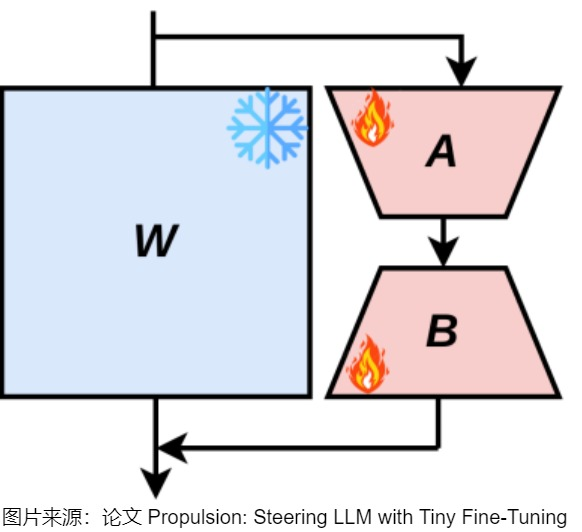
\includegraphics[width=0.35\textwidth]{img/09-ft-vs-lora.jpg}
	\end{center}

	\vspace{0.2cm}
	\begin{itemize}
		\item \textbf{Left (Full FT):} Update entire $d \times d$ weight matrix
		\item \textbf{Right (LoRA):} Freeze $W_0$, learn low-rank $\Delta W = BA$ where $B \in \mathbb{R}^{d \times r}$, $A \in \mathbb{R}^{r \times d}$
		\item Parameters: $d^2 \to 2rd$ (e.g., $4096^2 \to 2 \times 16 \times 4096 = 131K$)
	\end{itemize}

	\vspace{0.1cm}
	{\footnotesize Image credit: ``Exploring Transformer (22)---LoRA'' \cite{rossi2025lora}}
\end{frame}

% Slide 4b: LoRA Training Diagram
\begin{frame}{LoRA Training \& Inference}
	\begin{center}
		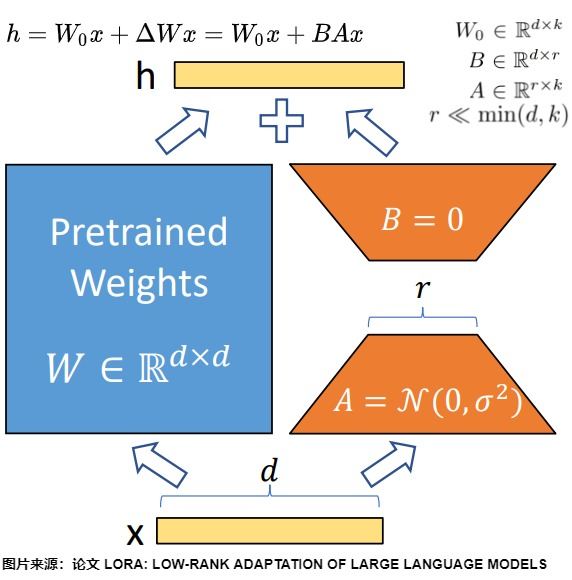
\includegraphics[width=0.25\textwidth]{img/09-lora-training.jpg}
	\end{center}


	\textbf{Training:} Freeze $W_0$, only update $A$ (Gaussian init) and $B$ (zero init).
	$$W_{\text{new}} = W_0 + \frac{\alpha}{r} \cdot BA$$

	\textbf{Inference:} Merge $W' = W_0 + \frac{\alpha}{r} BA$ --- zero overhead, same architecture.

		{\footnotesize Image credit: ``Exploring Transformer (22)---LoRA'' \cite{rossi2025lora}}
\end{frame}

% Slide 5: Efficient Computation
\begin{frame}{Efficient Computation}
	\textbf{Na\"ive approach:} Compute $\Delta W = AB^\top$ ($d \times k$), then $\Delta W \cdot x$.

	\vspace{0.2cm}
	\textbf{Efficient approach:} Reorder matrix multiplications:
	$$\underbrace{(xA)}_{\text{batch} \times r} \cdot B^\top \quad \text{instead of} \quad \underbrace{(AB^\top)}_{d \times k} \cdot x$$

	\vspace{0.3cm}
	\begin{table}
		\centering
		\small
		\begin{tabular}{lcc}
			\toprule
			\textbf{Method}                      & \textbf{FLOPs}    & \textbf{Intermediate Size} \\
			\midrule
			Na\"ive ($AB^\top$ then $\cdot x$)   & $dk + dk \cdot n$ & $d \times k$               \\
			Efficient ($xA$ then $\cdot B^\top$) & $dr + kr \cdot n$ & $n \times r$               \\
			\bottomrule
		\end{tabular}
	\end{table}

	\vspace{0.2cm}
	For $d = k = 4096$, $r = 16$, $n = 1$: efficient is $\sim 128\times$ less compute.

	\vspace{0.2cm}
	\textbf{Memory:} No need to materialize full $\Delta W$ matrix.
\end{frame}
% Slide 14b: A and B Matrix Roles
\begin{frame}{A and B Matrix: Asymmetric Roles}
	\begin{center}
		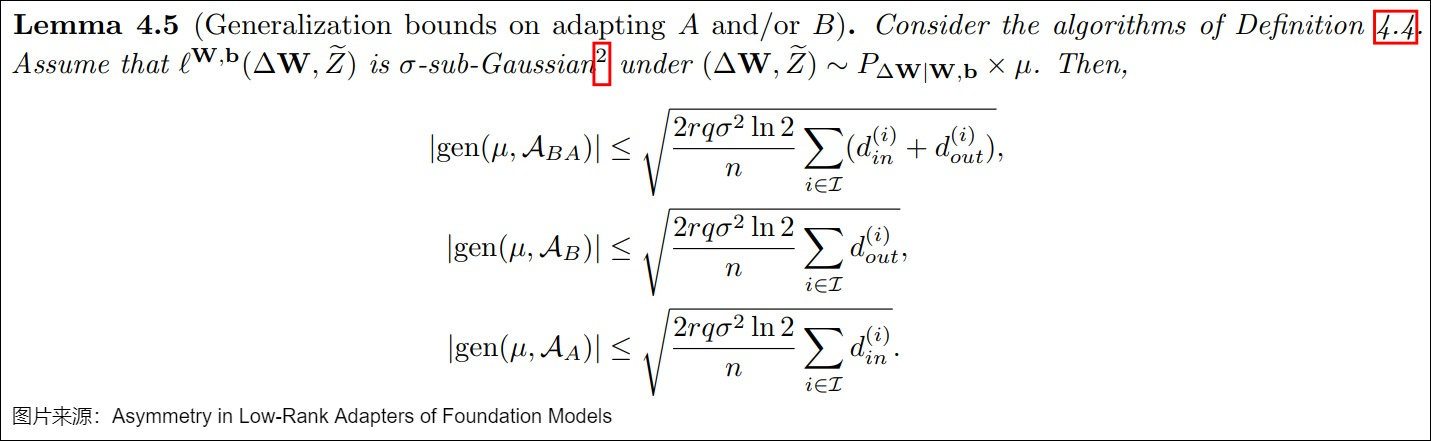
\includegraphics[width=0.65\textwidth]{img/09-ab-matrix.jpg}
	\end{center}

	\vspace{0.2cm}
	\begin{columns}
		\begin{column}{0.45\textwidth}
			\textbf{A matrix:} Feature extractor
			\begin{itemize}
				\item Captures cross-domain commonality
				\item Can be shared across tasks
				\item Less critical to update
			\end{itemize}
		\end{column}
		\begin{column}{0.5\textwidth}
			\textbf{B matrix:} Task adapter
			\begin{itemize}
				\item Captures task-specific differences
				\item More important than A
				\item Updating B alone $\approx$ full LoRA quality
			\end{itemize}
		\end{column}
	\end{columns}

	\vspace{0.1cm}
	{\footnotesize Image credit: ``Exploring Transformer (22)---LoRA'' \cite{rossi2025lora}}
\end{frame}

% Slide 6: Implementation - LoRA Layer
\begin{frame}[fragile]{Implementation: \texttt{LoRALayer}}
	\begin{lstlisting}[language=Python]
class LoRALayer(nn.Module):
    def __init__(self, in_dim, out_dim, rank, alpha=1.0, dropout=0.0):
        super().__init__()
        self.A = nn.Parameter(torch.randn(in_dim, rank) / math.sqrt(rank))
        self.B = nn.Parameter(torch.zeros(rank, out_dim))
        self.scaling = alpha / rank
        self.dropout = nn.Dropout(dropout)

    def forward(self, x):
        x = self.dropout(x)
        return (x @ self.A @ self.B) * self.scaling
    \end{lstlisting}

	\vspace{0.2cm}
	\textbf{Parameter count:} $r \times (d_{\text{in}} + d_{\text{out}})$

	\vspace{0.2cm}
	\textbf{Compression examples (512 $\to$ 256 layer):}
	\begin{itemize}
		\item $r=4$: 3,072 params vs 131,072 original ($42.7\times$ reduction)
		\item $r=16$: 12,288 params ($10.7\times$ reduction)
		\item $r=64$: 49,152 params ($2.7\times$ reduction)
	\end{itemize}
\end{frame}

% Slide 7: Integration with Existing Layers
\begin{frame}[fragile]{Integration with Existing Layers}
	\textbf{Wrapper pattern:} Freeze original weights, add LoRA branch.

	\begin{lstlisting}[language=Python]
class LinearWithLoRA(nn.Module):
    def __init__(self, linear_layer, rank, alpha=1.0):
        super().__init__()
        self.linear = linear_layer
        self.lora = LoRALayer(linear_layer.in_features,
                              linear_layer.out_features, rank, alpha)
        for param in self.linear.parameters():
            param.requires_grad = False

    def forward(self, x):
        return self.linear(x) + self.lora(x)
    \end{lstlisting}

	\vspace{0.2cm}
	\textbf{Design Principles:}
	\begin{itemize}
		\item \textbf{Frozen Base}: Original weights never change
		\item \textbf{Additive}: LoRA output added to original output
		\item \textbf{Selective}: Apply only to chosen layers
		\item \textbf{Composable}: Multiple adapters can be swapped
	\end{itemize}
\end{frame}

% Slide 8: Application Strategies
\begin{frame}{LoRA Application Strategies}
	\textbf{Where to apply LoRA in a network?}

	\vspace{0.3cm}
	\begin{table}
		\centering
		\small
		\begin{tabular}{lp{6cm}}
			\toprule
			\textbf{Strategy} & \textbf{Description}                          \\
			\midrule
			All Layers        & Apply LoRA to every linear layer              \\
			Output Only       & Only adapt the final classification layer     \\
			Input/Output      & Adapt first and last layers                   \\
			Attention Only    & Focus on Q, K, V, O projections               \\
			Selective         & Different ranks per layer based on importance \\
			\bottomrule
		\end{tabular}
	\end{table}

	\vspace{0.3cm}
	\textbf{Recommended for LLMs:} Target attention projections (Q, K, V, O) with optional MLP layers.

	\vspace{0.3cm}
	\textbf{Layer-specific ranks:}
	\begin{itemize}
		\item Larger / more important layers $\to$ higher rank
		\item Smaller / less critical layers $\to$ lower rank
	\end{itemize}
\end{frame}

% Slide 8b: LoRA Placement in Transformer
\begin{frame}{Where to Place LoRA in Transformer?}
	\begin{columns}
		\begin{column}{0.55\textwidth}
			\begin{center}
				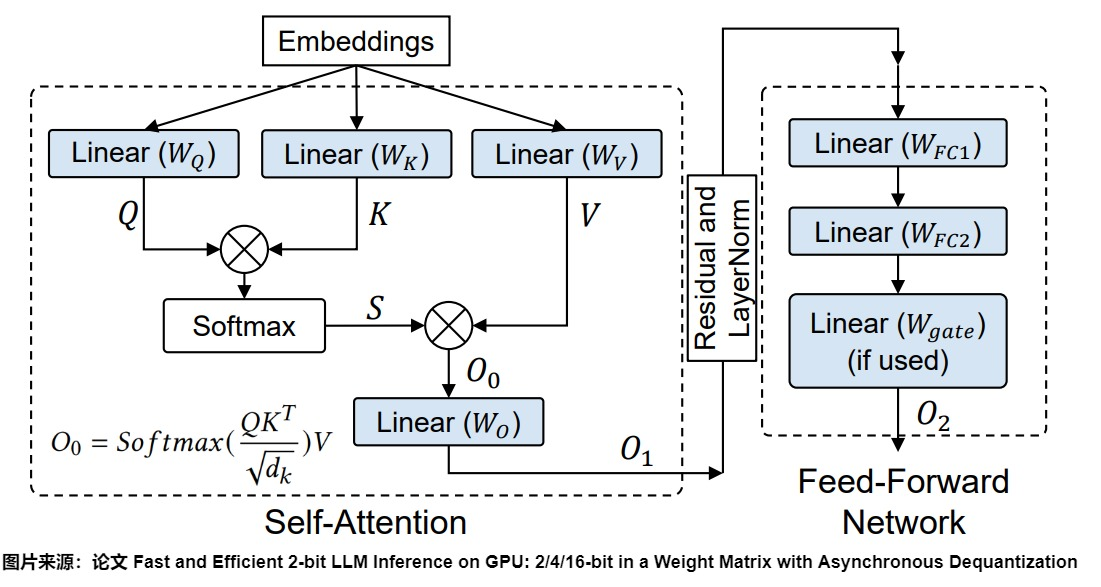
\includegraphics[width=\textwidth]{img/09-dense-layers.jpg}
			\end{center}
			{\footnotesize Blue boxes = dense layers suitable for LoRA}
		\end{column}
		\begin{column}{0.42\textwidth}
			\textbf{Dense layers in Transformer:}
			\begin{itemize}
				\item \textbf{Attention:} $W^Q$, $W^K$, $W^V$, $W^O$
				\item \textbf{FFN (MLP):} gate\_proj, up\_proj, down\_proj
			\end{itemize}

			\vspace{0.2cm}
			\textbf{Original LoRA paper:} Only $W^Q$ and $W^V$

			\vspace{0.2cm}
			\textbf{Best practice:} All 4 attention projections (+ optionally FFN)
		\end{column}
	\end{columns}

	\vspace{0.1cm}
	{\footnotesize Image credit: ``Exploring Transformer (22)---LoRA'' \cite{rossi2025lora}}
\end{frame}

% Slide 8c: PEFT Taxonomy
\begin{frame}{PEFT Methods Taxonomy}
	\begin{center}
		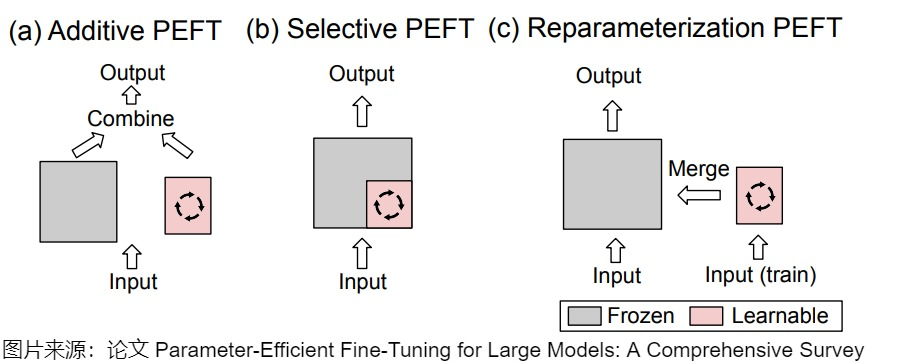
\includegraphics[width=0.75\textwidth]{img/09-peft-taxonomy.jpg}
	\end{center}

	\vspace{0.2cm}
	\textbf{LoRA belongs to ``Reparameterization PEFT''} --- builds low-dimensional reparameterization of original weights.

	\vspace{0.1cm}
	Other categories: Additive (adapters, prompts), Selective (freeze subsets), Hybrid (combine methods).

		{\footnotesize Image credit: ``Exploring Transformer (22)---LoRA'' \cite{rossi2025lora}}
\end{frame}

% Slide 9: PEFT Library
\begin{frame}[fragile]{HuggingFace PEFT Library}
	\textbf{PEFT} (Parameter-Efficient Fine-Tuning) is the industry standard for LoRA on LLMs.

	\vspace{0.3cm}
	\textbf{One-Line LoRA:}
	\begin{lstlisting}[language=Python]
from peft import LoraConfig, get_peft_model
config = LoraConfig(
    task_type=TaskType.CAUSAL_LM,
    r=16, lora_alpha=32, lora_dropout=0.05,
    target_modules=['q_proj', 'k_proj', 'v_proj', 'o_proj'],
)
peft_model = get_peft_model(base_model, config)
    \end{lstlisting}

	\vspace{0.2cm}
	\textbf{Key configuration:}
	\begin{itemize}
		\item \texttt{r}: Rank (typically 8--64)
		\item \texttt{lora\_alpha}: Scaling factor (typically $2r$)
		\item \texttt{target\_modules}: Which layers get LoRA adapters
		\item \texttt{task\_type}: CAUSAL\_LM, SEQ\_CLS, etc.
	\end{itemize}
\end{frame}

% Slide 10: PEFT on Qwen2.5
\begin{frame}{LoRA on Qwen2.5-0.5B}
	\textbf{Base model:} Qwen2.5-0.5B (Alibaba) --- 24 layers, 896 hidden dim

	\vspace{0.3cm}
	\begin{table}
		\centering
		\small
		\begin{tabular}{lrr}
			\toprule
			\textbf{Module} & \textbf{Shape} & \textbf{LoRA Target?} \\
			\midrule
			q\_proj         & $896 \to 896$  & \checkmark            \\
			k\_proj         & $896 \to 128$  & \checkmark            \\
			v\_proj         & $896 \to 128$  & \checkmark            \\
			o\_proj         & $896 \to 896$  & \checkmark            \\
			gate\_proj      & $896 \to 4864$ & optional              \\
			up\_proj        & $896 \to 4864$ & optional              \\
			down\_proj      & $4864 \to 896$ & optional              \\
			\bottomrule
		\end{tabular}
	\end{table}

	\vspace{0.2cm}
	\textbf{Result with $r=16$ on attention projections:}
	\begin{itemize}
		\item Total params: 494M
		\item Trainable params: 2.16M
		\item \textbf{229$\times$ parameter reduction} (0.44\% trainable)
	\end{itemize}
\end{frame}

% Slide 11: SFT with LoRA
\begin{frame}{Supervised Fine-Tuning with LoRA}
	\textbf{Training workflow:}
	\begin{enumerate}
		\item Load instruction dataset (e.g., medical QA)
		\item Format into instruction-response pairs
		\item Train \textbf{only LoRA parameters} (base weights frozen)
		\item Monitor loss convergence
	\end{enumerate}

	\vspace{0.3cm}
	\begin{block}{Training Configuration}
		\begin{itemize}
			\item Optimizer: AdamW (lr=$2 \times 10^{-4}$, weight\_decay=0.01)
			\item Gradient clipping: max\_norm=1.0
			\item Only LoRA params receive gradients
		\end{itemize}
	\end{block}

	\vspace{0.2cm}
	\textbf{Observed results (medical QA, 10 epochs):}
	\begin{itemize}
		\item Initial loss: 2.71 $\to$ Final loss: 0.31 (88.5\% reduction)
		\item Model learns task-specific patterns through LoRA adapters
	\end{itemize}
\end{frame}



% Slide 14: LoRA Variants
\begin{frame}{LoRA Variants: DoRA and rsLoRA}
	\textbf{Drop-in improvements over standard LoRA:}


	\begin{block}{DoRA (Weight-Decomposed LoRA, 2024)}
		Decomposes weight into \textbf{magnitude} and \textbf{direction}:
		$$W' = m \cdot \frac{W + AB^\top}{\|W + AB^\top\|}$$
		\begin{itemize}
			\item Learnable magnitude vector $m$ . Better performance at low ranks
			\item Slightly more parameters ($+$ magnitude vector)
		\end{itemize}
	\end{block}


	\begin{block}{rsLoRA (Rank-Stabilized LoRA, 2024)}
		Scaling factor: $\alpha / \sqrt{r}$ instead of $\alpha / r$
		\begin{itemize}
			\item More stable training across different rank values
			\item Higher ranks maintain stronger adaptation
		\end{itemize}
	\end{block}
\end{frame}



% Slide 15: Variant Comparison
\begin{frame}{Variant Comparison}
	\begin{table}
		\centering
		\small
		\begin{tabular}{llcc}
			\toprule
			\textbf{Variant} & \textbf{Scaling}    & \textbf{Extra Overhead} & \textbf{Best For}   \\
			\midrule
			Standard LoRA    & $\alpha / r$        & none                    & General purpose     \\
			rsLoRA           & $\alpha / \sqrt{r}$ & none                    & High rank scenarios \\
			DoRA             & $\alpha / r$        & magnitude vec.          & Low rank scenarios  \\
			\bottomrule
		\end{tabular}
	\end{table}

	\vspace{0.3cm}
	\textbf{Qwen2.5-0.5B comparison ($r=16$, $\alpha=32$):}
	\begin{table}
		\centering
		\small
		\begin{tabular}{lrl}
			\toprule
			\textbf{Variant} & \textbf{Trainable Params} & \textbf{Scaling Factor}  \\
			\midrule
			Standard LoRA    & 2,162,688                 & $\alpha/r = 2.00$        \\
			rsLoRA           & 2,162,688                 & $\alpha/\sqrt{r} = 8.00$ \\
			DoRA             & 2,211,840                 & $\alpha/r = 2.00$        \\
			\bottomrule
		\end{tabular}
	\end{table}

	\vspace{0.2cm}
	\textbf{All variants are drop-in replacements --- just change \texttt{LoraConfig} flags!}
\end{frame}

% Slide 16: Adapter Workflow
\begin{frame}[fragile]{Production Workflow: Save, Load, Merge}
	\textbf{Critical for deployment:}

	\vspace{0.3cm}
	\begin{enumerate}
		\item \textbf{Save}: Store only adapter weights (tiny: $\sim$MB vs $\sim$GB for full model)
		\item \textbf{Load}: Reuse adapter on same or different base model
		\item \textbf{Merge}: Combine $W' = W + \frac{\alpha}{r} AB^\top$ into base model --- zero inference overhead
		\item \textbf{Multi-adapter}: Hot-swap task-specific adapters at runtime
	\end{enumerate}

	\vspace{0.3cm}
	\begin{block}{Storage Example}
		\begin{itemize}
			\item 100 task-specific adapters: $\sim$100 MB total
			\item 100 full fine-tuned models: $\sim$100 GB total
			\item \textbf{1000$\times$ storage savings!}
		\end{itemize}
	\end{block}

	\vspace{0.2cm}
	\begin{lstlisting}[language=Python]
model.save_pretrained('./my_adapter')
loaded = PeftModel.from_pretrained(base, './my_adapter')
merged = loaded.merge_and_unload()
    \end{lstlisting}
\end{frame}

% Slide 17: When to Use What
\begin{frame}{Decision Guide: When to Use What?}
	\begin{table}
		\centering
		\small
		\begin{tabular}{p{3.5cm}p{3.5cm}p{4cm}}
			\toprule
			\textbf{Scenario}    & \textbf{Method}     & \textbf{Reason}          \\
			\midrule
			Plenty of GPU memory & Full fine-tuning    & Best quality             \\
			Limited GPU memory   & LoRA ($r=16$--$64$) & Good quality, low memory \\
			Very limited memory  & QLoRA (4-bit)       & Minimum memory           \\
			Low-rank tasks       & DoRA                & Better at low $r$        \\
			High-rank tasks      & rsLoRA              & Stable scaling           \\
			Multi-task serving   & LoRA + hot-swap     & One base, many adapters  \\
			Edge deployment      & Merge LoRA          & Zero overhead            \\
			\bottomrule
		\end{tabular}
	\end{table}

	\vspace{0.3cm}
	\textbf{Typical starting point for LLMs:}
	\begin{itemize}
		\item $r = 16$, $\alpha = 32$ (scaling = 2.0)
		\item Target: Q, K, V, O projections (+ optionally MLP layers)
		\item Dropout: 0.05
		\item Learning rate: $2 \times 10^{-4}$ to $3 \times 10^{-4}$
	\end{itemize}
\end{frame}

% Slide 18: Lab Implementation
\begin{frame}[fragile]{Lab: What You'll Implement}
	\textbf{Part 1: LoRA from Scratch}
	\begin{itemize}
		\item Build \texttt{LoRALayer} with proper initialization ($A \sim \mathcal{N}$, $B = 0$)
		\item Build \texttt{LinearWithLoRA} wrapper with frozen base weights
		\item Test different rank/alpha configurations
		\item Apply to multi-layer network with various strategies
	\end{itemize}

	\vspace{0.2cm}
	\textbf{Part 2: PEFT on Real LLMs}
	\begin{itemize}
		\item Load Qwen2.5-0.5B with \texttt{transformers}
		\item Apply LoRA via \texttt{get\_peft\_model()}
		\item Fine-tune on medical QA dataset
		\item Test QLoRA with 4-bit NF4 quantization
	\end{itemize}

	\vspace{0.2cm}
	\textbf{Part 3: Production Workflow}
	\begin{itemize}
		\item Save/load adapters
		\item Merge LoRA into base model
		\item Compare DoRA vs rsLoRA vs standard LoRA
	\end{itemize}
\end{frame}

% Slide 19: Summary
\begin{frame}{Summary: Key Takeaways}
	\begin{enumerate}
		\item \textbf{LoRA Core}: $\Delta W = AB^\top$ with $r \ll \min(d, k)$
		      \begin{itemize}
			      \item 100--1000$\times$ parameter reduction
			      \item $B=0$ initialization ensures stable start
		      \end{itemize}

		\item \textbf{Efficient Computation}: $(xA)B^\top$ avoids materializing full $\Delta W$

		\item \textbf{Integration}: Freeze base weights, add LoRA branch, train only adapters

		\item \textbf{PEFT}: One-line LoRA for any HuggingFace model

		\item \textbf{QLoRA}: 4-bit NF4 + LoRA = fine-tune 7B on 6 GB VRAM

		\item \textbf{Variants}: DoRA (weight-decomposed), rsLoRA (rank-stabilized)

		\item \textbf{Production}: Save/load adapters (MB), merge for zero-overhead inference
	\end{enumerate}
\end{frame}

% Slide 20: Resources
\begin{frame}{Resources}
	\begin{itemize}
		\item \textbf{LoRA Paper}: Hu et al., ``LoRA: Low-Rank Adaptation of Large Language Models'' (2021) \\
		      \href{https://arxiv.org/abs/2106.09685}{arXiv:2106.09685}

		\item \textbf{QLoRA Paper}: Dettmers et al., ``QLoRA: Efficient Finetuning of Quantized LLMs'' (2023) \\
		      \href{https://arxiv.org/abs/2305.14314}{arXiv:2305.14314}

		\item \textbf{DoRA Paper}: Liu et al., ``DoRA: Weight-Decomposed Low-Rank Adaptation'' (2024) \\
		      \href{https://arxiv.org/abs/2402.09353}{arXiv:2402.09353}

		\item \textbf{rsLoRA}: Kalajdzievski, ``A Rank Stabilization Scaling Factor for Fine-Tuning with LoRA'' (2024) \\
		      \href{https://arxiv.org/abs/2312.03732}{arXiv:2312.03732}

		\item \textbf{HuggingFace PEFT}: \href{https://github.com/huggingface/peft}{github.com/huggingface/peft}

		\item \textbf{Blog Reference}: ``Exploring Transformer (22)---LoRA'' (RossiXYZ, 2025) \\
		      \href{https://www.cnblogs.com/rossiXYZ/p/18805103}{cnblogs.com/rossiXYZ/p/18805103}

		\item \textbf{Lab Notebook}: \texttt{LLM09-LoRA-Fine-Tuning.ipynb}
	\end{itemize}
\end{frame}

\begin{thebibliography}{9}
	\bibitem{rossi2025lora}
	RossiXYZ, ``Exploring Transformer (22)---LoRA,'' Cnblogs Blog, Apr. 2025.
	\href{https://www.cnblogs.com/rossiXYZ/p/18805103}{cnblogs.com/rossiXYZ/p/18805103}

	\bibitem{hu2021lora}
	E.~J. Hu \emph{et al.}, ``LoRA: Low-Rank Adaptation of Large Language Models,'' \emph{arXiv preprint arXiv:2106.09685}, 2021.

	\bibitem{dettmers2023qlora}
	T.~Dettmers \emph{et al.}, ``QLoRA: Efficient Finetuning of Quantized LLMs,'' \emph{arXiv preprint arXiv:2305.14314}, 2023.

	\bibitem{liu2024dora}
	S.~Liu \emph{et al.}, ``DoRA: Weight-Decomposed Low-Rank Adaptation,'' \emph{arXiv preprint arXiv:2402.09353}, 2024.

	\bibitem{kalajdzievski2024rslora}
	D.~Kalajdzievski, ``A Rank Stabilization Scaling Factor for Fine-Tuning with LoRA,'' \emph{arXiv preprint arXiv:2312.03732}, 2024.
\end{thebibliography}

\end{document}
